\chapter{Liveness of Bitcoin}
The last lecture focused on the safety of the longest chain protocol, which is a rule that determines which block is the valid one in the case of a fork. The safety property means that once a block is confirmed by being k-deep in the chain, then the probability of it being deconfirmed by another fork is very small, as long as k is large enough. This ensures that the blockchain does not have conflicting histories, and that users can trust the transactions that are recorded in it.\\\\
We are interested in exploring the scenarios where the ledger does not receive any new blocks, or where some transactions from honest users are excluded from the blocks. 
\section{What is Liveness}
Liveness is a term that describes the ability of a blockchain protocol to ensure that the transactions that are submitted by honest users are eventually included in the ledger, and that the blocks that contain these transactions are part of the longest chain. Liveness is an important security property because it guarantees that the network will not stop producing new blocks and confirming transactions, and that users can use the system without delays or failures. Liveness also prevents the network from being stuck in a fork, where different nodes have different views of the ledger.\\\\
Both liveness and safety are essential for a blockchain protocol to function properly and securely. A good consensus protocol should achieve both liveness and safety under reasonable assumptions about the network and the participants. However, there is often a trade-off between liveness and safety, as increasing one may decrease the other. For example, requiring more confirmations for a block to be considered final may increase safety, but it may also increase latency and reduce liveness. Therefore, finding the optimal balance between liveness and safety is a challenging task for blockchain protocol designers.\\\\
Liveness is definitely compromised if there is a deadlock. A deadlock occurs when the protocol gets stuck and the miners and parties cannot perform their tasks and mine new blocks.\\
 The longest chain protocol cannot deadlock, which means that it will always produce a unique longest chain, even if there are multiple forks. This ensures that the network can always reach a consensus on the state of the ledger, and that users can always find the valid block.\\
The mining operation is very democratic, which means that any honest miner with a small amount of hash power can eventually succeed in mining a block and adding it to the chain. This encourages participation and decentralization in the network, and prevents monopoly or censorship by powerful miners.\\\\
There are two adversarial events that can threaten liveness:
\begin{enumerate}
    \item All blocks on the longest chain are mined by an adversary
    \item An adversary mines a block that is empty or censors specific transactions.
\end{enumerate} 
We need to examine Chain Quality, which is based on Chain Growth, to determine the likelihood of an honest miner’s block being left out of the longest chain or under what circumstances this occurs.

\section{Chain Growth}
\dfn{Chain Growth}{Chain growth is defined as the rate of growth of the longest chain, denoted by CG.}
If there is no fork in the chain, and only the longest chain exists, then its growth rate depends on the difficulty level, and it adds one block every 10 minutes on average.  But it slows down for two reasons :
\begin{enumerate}
    \item Not all miners may be behaving safely.
    \item It could be that they're working in parallel
\end{enumerate}
The chain keeps growing and new blocks are continuously added to the longest chain because of positive chain growth. An honest miner has a chance to mine a block, even if it is small because the mining operation is random.\\\\
Chain growth depends on the behavior of the adversary, who controls a fraction of the hash power in the network, denoted by $\beta$. If the adversary stays silent, which means that he does not mine or broadcast any blocks, then chain growth is equal to the rate of block production by the honest nodes :
\begin{align*}
    CG=\frac{(1-\beta)\lambda}{1+(1-\beta)\lambda\Delta}
\end{align*}
One can see that the adversary really cannot do anything better than this. Delivering an honest block earlier than $\Delta$ time or publishing any adversarial block will just increase the chain growth. Therefore, we have the bound:
\begin{align}
    CG\ge \frac{(1-\beta)\lambda}{1+(1-\beta)\lambda\Delta}
    \label{eq1}
\end{align}
 If the adversary acts honestly, which means that he mines and broadcasts blocks according to the protocol rules, then chain growth is equal to :
 \begin{align*}
    CG=\frac{(1-\beta)\lambda}{1+(1-\beta)\lambda\Delta} + \beta\lambda
 \end{align*}
\begin{figure}[h!]
    \centering
    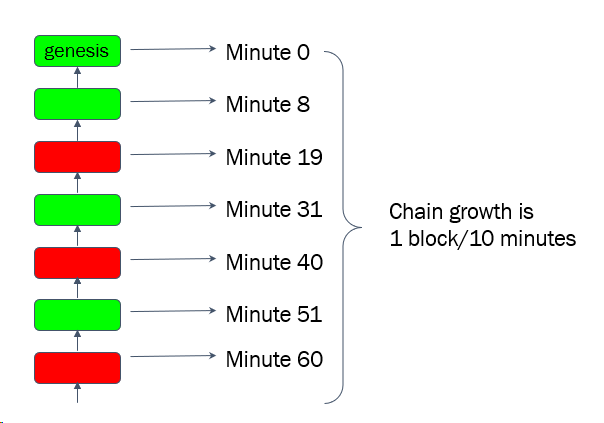
\includegraphics[width=0.5\linewidth]{Fig/07/F1}
    \caption{Chain Growth}
    \label{fig:f1}
\end{figure}
\section{Chain Quality}
\dfn{Chain Quality}{We define the chain quality of a longest chain C as the fraction of honest blocks in C, denoted as CQ
\begin{align*}
    CQ = \frac{\text{\# of honest blocks in the longest chain}}{\# \text{ of all blocks in the longest chain}}
\end{align*}}
Positive chain quality ensures that a positive fraction of blocks mined by honest nodes enters the longest chain. Having enough blocks mined by honest nodes on the longest chain (i.e., high CQ) ensures that transactions enter the blockchain at a fast clip – thus CQ helps quantify the level of liveness.\\\\
Furthermore, CQ quantifies fairness: since block rewards are provided to blocks in the longest chain, having blocks mined by honest nodes in the longest chain ensures that honest miners are rewarded.
\begin{figure}[h!]
    \centering
    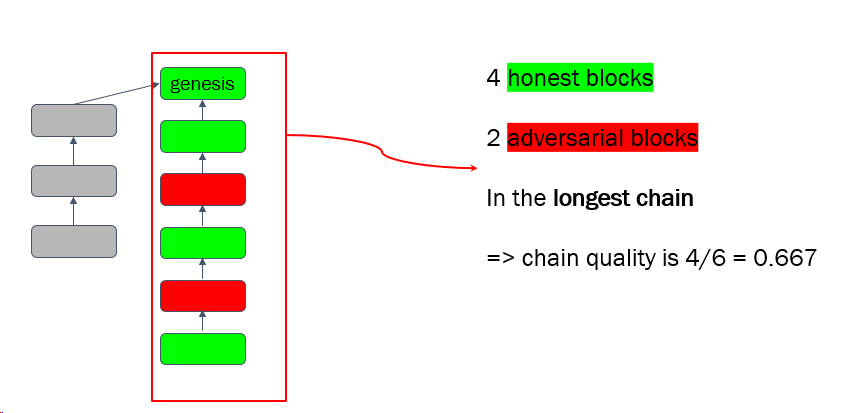
\includegraphics[width=0.7\linewidth]{Fig/07/F2}
    \caption{Chain Quality}
    \label{fig:f2}
\end{figure}\\
Positive chain growth and positive chain quality are together combined to ensure that any honest transaction will
eventually be added to a block on the longest chain and to the ledger, which gives us liveness.\\\\
If the chain growth is CG and the adversary can mine blocks at a rate of at most $\beta\lambda$, by the definition of the chain quality, we have a lower bound:
\begin{align}
    CQ \ge \frac{CG \times T - \beta\lambda T}{CG \times T} = \frac{CG - \beta\lambda}{CG}
    \label{eq2}
\end{align}
Plugging \ref{eq1} in \ref{eq2} :
\begin{align*}
    CQ > 0 \Leftrightarrow \frac{(1-\beta)\lambda}{1+(1-\beta)\lambda\Delta} > \beta\lambda
\end{align*}
This is exactly the same threshold as the safety guarantee as we have seen before. Therefore, we can conclude the following security guarantee on the longest chain protocol.
\thm{}{The longest chain protocol is safe and live, exactly under the following condition:
\begin{align*}
    \frac{1-\beta}{1+(1-\beta)\Delta} > \beta
\end{align*}}

\section{Selfish Mining}
The ideal chain quality is when the number of honest blocks on the longest chain is proportional to the honest hash power, which is $CQ = 1 - \beta$. However, this does not happen in the longest chain protocol because of \textbf{selfish mining}, which is a strategy where an adversary tries to create a private fork and withhold it from the network until he can overtake the public chain. \\\\\
Consider the following adversarial strategy :
\begin{itemize}
    \item The adversary always mines on the block at the tip of the longest chain, whether the chain is private or public. Upon successful mining, the adversary maintains the block in private to release it at an appropriate time.
    \item When an honest miner publishes a block the adversary will release a previously mined block
    at the same level (if it has one). We assume that the adversary can break ties in its favor, so
    honest miners will mine on the adversarial block.
\end{itemize}
\begin{figure}[h!]
    \centering
    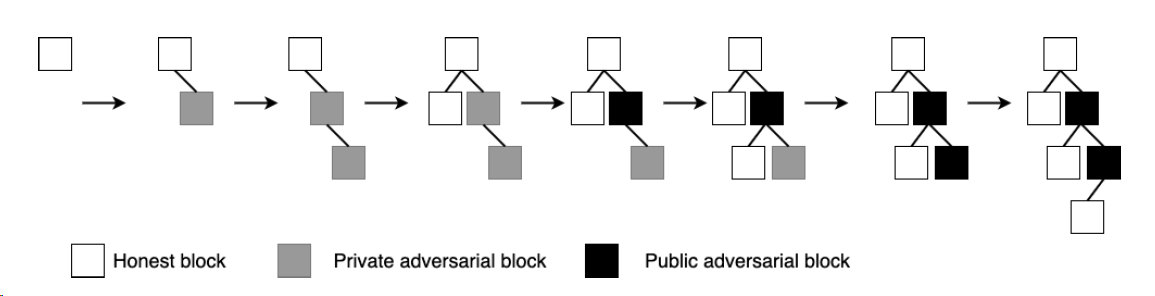
\includegraphics[width=0.7\linewidth]{Fig/07/F3}
    \caption{Selfish mining example}
    \label{fig:f3}
\end{figure}
Selfish mining reduces the chain quality and liveness of the protocol, and gives an unfair advantage to the adversary.

\section{Fruitchains}
The longest chain protocol would have the best possible chain quality, $CQ = 1 - \beta$, if the adversary followed the protocol rules. But what if the adversary tries to cheat and disrupt the protocol? Can we design a better protocol that can achieve the optimal chain quality no matter what the adversary does? And can we do it with only a minor change to the longest chain protocol?\\ \textbf{Fruitchains} is a protocol that does exactly that. It achieves the optimal chain quality, and it does it fast.\\\\
The longest chain protocol links the security and the rewards of a block. The more blocks are built on top of a block, the safer and more profitable it is. Fruitchains is a new protocol that separates these two aspects by using two different types of blocks:
\begin{itemize}
    \item \textbf{transaction block}, which has all the transactions (or data) that a block in the longest chain protocol would have.
    \item \textbf{proposer block}, which has only the header information that a block in the longest chain protocol would have.
\end{itemize}
\begin{figure}[h!]
    \centering
    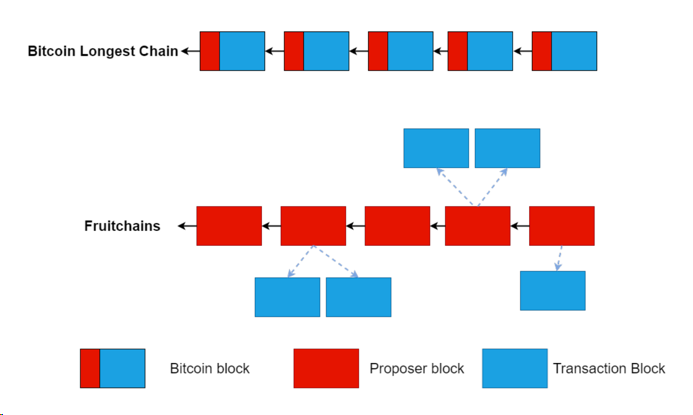
\includegraphics[width=0.7\linewidth]{Fig/07/F4}
    \caption{Comparison between blocks in the longest chain protocol and the transaction and proposer
        blocks in Fruitchains.}
    \label{fig:f4}
\end{figure}

These two types of blocks need to be linked and coupled together in a secure way. This is done by putting the hash of each transaction block inside a proposer block (see Figure \ref{fig:f4}). The two types of blocks are also connected during the mining process by using “2 for 1 mining”, also known as \textbf{cryptographic sortition}.

\subsection{Cryptographic Sortition}
In the mining process, the two types of blocks – transaction and proposer blocks – are mined together. A miner first creates a \textbf{superblock}, which is similar to a normal block in the longest chain protocol. The superblock has two parts: a transaction block and a proposer block. But that’s where the similarity ends.\\
We say a superblock is successfully mined if 
\begin{align*}
    Hash(\text{nonce}, \text{superblock}) < T_{tx} + T_{prop} 
\end{align*}
The mining process determines whether a superblock is a transaction block or a proposer block based on the hash output:
\begin{itemize}
    \item If the hash output is smaller than $T_{prop}$, the superblock is a proposer block.
    \item If the hash output is between $T_{prop}$ and $T_{tx} + T_{prop}$, the superblock is a transaction block.
\end{itemize}
\begin{figure}[h!]
    \centering
    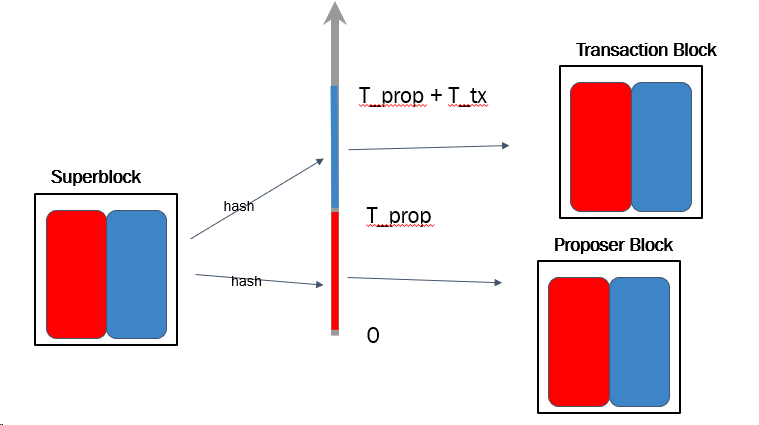
\includegraphics[width=0.5\linewidth]{Fig/07/F5}
    \caption{Superblock}
    \label{fig:f5}
\end{figure}
The hash functions produce random outputs, so the chance of a superblock being a proposer or a transaction block depends on $T_{prop}$ or $T_{tx}$, respectively. This means that two different kinds of blocks are mined together, but only one of them is chosen as the result of the mining process. This is called “two-for-one mining” or “cryptographic sortition”.
\subsection{Fruitchain Protocol}
The ledger is a list of transactions that are sorted by some rules. The rules are:
\begin{itemize}
    \item First, sort the proposer blocks by using the longest chain rule, which means that the valid chain is the one with the most blocks.
    \item Second, sort the transaction blocks that each proposer block refers to. For example, you can sort them by their hash value, which is a unique code for each block.
    \item Third, sort the transactions in each transaction block. For example, you can sort them by using the lexicographic ordering of the transactions in the Merkle tree representation, which is a way of organizing the transactions in a tree shape.
\end{itemize}
\subsubsection{Safety of fruitchain protocol}
Assuming $\lambda_{tx}$ and $\lambda_{prop}$ as the mining rate of the transaction blocks and proposer blocks respectively;
these mining rates are directly proportional to the difficulty targets $T_{tx}$ and $T_{prop}$, respectively.
The safety of this protocol follows directly from the safety of the longest chain protocol: as long as
$\lambda_{prop}$ is small enough, i.e.,
\begin{align*}
    \frac{1-\beta}{1+(1-\beta)\lambda_{prop}\Delta} > \beta
\end{align*}
The $k$-deep proposer block in the longest chain will be permanent with high probability (for large
enough k). This stabilizes the ledger guaranteeing safety.
\subsubsection{Liveness of fruitchain protocol}
We want to show that the optimal CQ of $1 − \beta$ is achieved no matter what the adversary does to interfere with the transaction and proposer block mining. We start by looking at the selfish mining attack: suppose an adversary tries to hide some proposer blocks that were mined by an honest party (and that contain some honest transaction blocks) by mining on a secret branch. Then, by the liveness property of the longest chain protocol (which guarantees positive CQ and CG), sooner or later an honest party will mine a new proposer block that includes those displaced transaction blocks. And if k is large enough, this proposer block will be securely added to the ledger.\\\\
We know that the honest and adversarial parties mine transaction blocks according to Poisson processes with rates $(1 − \beta)\lambda_{tx}$ and $\beta\lambda_{tx}$ respectively. And by the liveness property of the longest chain protocol, every honest transaction block will eventually be part of the proposer chain. Therefore, by considering an average on the entire longest proposer chain, we have
\begin{align*}
    CQ \ge \frac{(1-\beta)\lambda_{tx}}{(1-\beta)\lambda_{tx} + \beta\lambda_{tx}} = 1 - \beta
\end{align*}
Note that here we define chain quality as the fraction of honest transaction blocks instead of honest proposer blocks, and further determining mining rewards by transaction block yields fair rewards.

\subsection{Short time scale optimal CQ}
The protocol is not secure in a short time span, because a private block attacker could secretly mine many transaction blocks and release them all at once, making a large portion of the proposer chain consist of adversarial transaction blocks.\\\\
This issue is resolved by making sure that a transaction block is attached to a proposer block that is close enough to the proposer block that includes it. Each transaction block has two parent blocks:
\begin{itemize}
    \item A confirmed parent, which is a proposer block that has been stabilized/confirmed (i.e., k-deep block) and that the transaction block hangs from.
    \item A proposer parent, which should be the tip of the longest proposer chain.
\end{itemize}
Note that a proposer block also has a confirmed parent, because the two-for-one mining process links the transaction block mining and the proposer block mining.\\\\
\begin{figure}[h!]
    \centering
    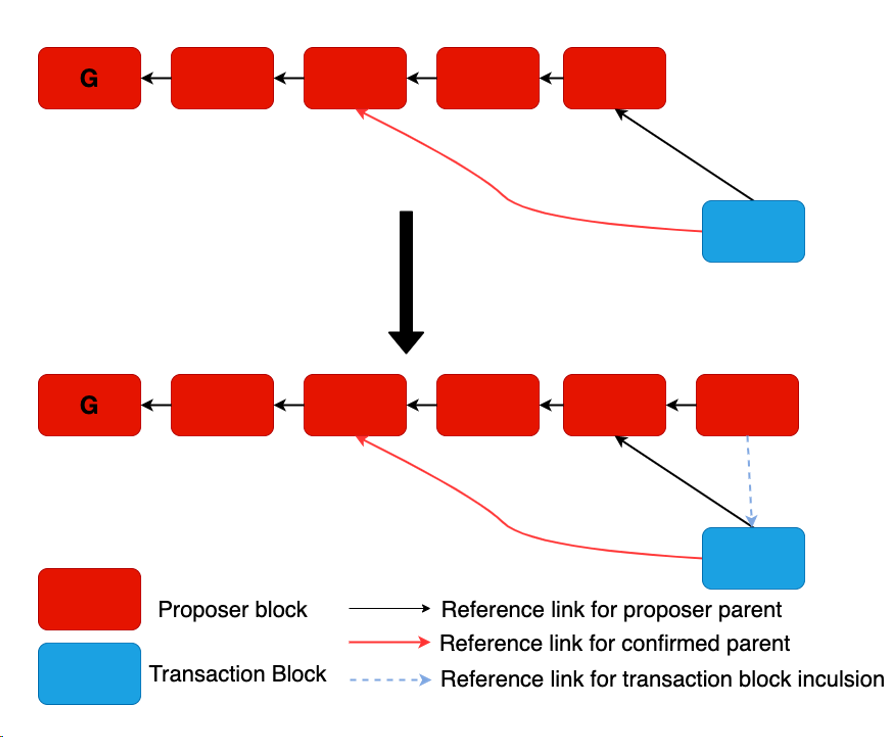
\includegraphics[width=0.6\linewidth]{Fig/07/F6}
    \caption{Fruitchain protocol}
    \label{fig:f6}
\end{figure}
A transaction block $B_{tx}$ is recent with respect to a proposer chain $C$ if its confirmed parent is not too far from the tip of $C$. The distance is measured by the recency parameter $R$, which is a fixed number. We achieve our goal by only allowing proposer blocks to include recent transaction blocks. By choosing a large enough $R$, we make sure that any transaction block mined by an honest party will be deep enough in the proposer chain. So, the optimal $CQ$ property still holds. Moreover, since only fresh transaction blocks can be included, the optimal $CQ$ is achieved even for short parts of the longest chain.
